\chapter{Cơ sở lý thuyết và các nghiên cứu liên quan}
\label{chapter2}
\section{ Kiểm thử thâm nhập}
\subsection{Tổng quan}

Như đã trình bày tại \textbf{Chương \ref{chapter1}}, dữ liệu ngày nay là tài sản, tài nguyên vô cùng quan trọng. Ngày càng nhiều những thông tin mật, tuyệt mật và riêng tư được lưu trữ trên hệ thống máy tính, nơi thông thường đều được kết nối mạng. Những thông tin này bao gồm rất nhiều lĩnh vực khác nhau như kinh tế, tài chính, y tế, giáo dục, khoa học, thậm chí là quân sự. Giá trị của những thông tin này không thể đong đếm được. Thách thức đặt ra là phải bảo vệ những thông tin này an toàn. Nếu dữ liệu được lưu trữ trong một hệ thống máy tính, bằng cách nào đó, hệ thống này phải được chứng minh rằng nó đủ an toàn và không dễ bị tấn công. Diễn tập hay thử nghiệm các bài tất công có chủ đích như là một phương pháp đắc lực, hiệu quả và có thể xác nhận.

\subsection{Phương pháp tiếp cận}

Kiểm thử xâm nhập là một cách tiếp cận để tăng cường và củng cố an ninh của hệ thống thông tin, nhưng nó chắc chắn không nói lên rằng hệ thống là hoàn toàn bất khả xâm phạm. Thông thường sẽ được thực hiện theo những kịch bản có sẵn với một danh sách các lỗi đã được công bố.

Hiện nay, có nhiều phương pháp hỗ trợ kiểm thử xâm nhập. Đây vừa là thuận lợi, vừa cũng là khó khăn khi đòi hỏi người thực hiện phải chọn phương pháp phù hợp. Người kiểm thử càng có nhiều kinh nghiệm, càng có nhiều kiến thức tốt hơn về môi trường được kiểm tra thì càng có thể đưa ra lựa chọn chính xác hơn về một phương pháp phù hợp, chẳng hạn như Open Source Security Testing Methodology Manual do ISECOM tạo và duy trì hoặc Open Web Application Security Project (OWASP) đối với các ứng dụng web và phần mềm. 

Đối với OWASP, đây là một dự án được tạo ra và duy trì bởi OWASP - một tổ chức phi lợi nhuận gồm có nhiều thành viên là các chuyên gia từ ngành phát triển ứng dụng web hoặc các chuyên gia trong lĩnh vực phần mềm. OWASP hướng tới phương pháp xây dựng những ứng dụng và dịch vụ web một cách an toàn, bằng cách mô tả những gì cần làm tại mỗi giai đoạn phát triển phần mềm để có thể đạt được mục tiêu là sự an toàn nhất có thể cho sản phẩm. Ngoài ra, OWASP cũng cung cấp một báo cáo được cập nhật thường xuyên về các nguy cơ bảo mật đối với bảo mật ứng dụng web, tập trung vào 10 rủi ro, lỗ hổng quan trọng và phổ biến nhất, được gọi là OWASP TOP 10.

OWASP đưa ra một quy trình hoặc kiến trúc của một bài kiểm tra xâm nhập phần mềm, thường chia ra làm nhiều giai đoạn. Trong đó, mỗi kết quả của giai đoạn này chính là đầu vào cho giai đoạn tiếp theo. Trong tình huống thực tế cụ thể, những giai đoạn này lại chia thành nhiều bước khác nhau để đánh giá logic của hệ thống được kiểm tra.

Các bước cụ thể có thể khác nhau, nhưng nhìn chung, chúng phải trải qua các giai đoạn sau.
\begin{itemize}
    \item Thu thập thông tin: thực hiện tìm kiếm, quét hệ thống, phần mềm, người sử dụng phần mềm, người vận hành hệ thống. Mục đích là tìm ra một lỗ hổng trong hệ thống.
    \item Dựa vào lỗ hổng đã được khám phá, tiến hành tần công thâm nhập hệ thống, mục đích là có được quyền quản trị hệ thống, tiếp tục sử dụng quyền mới để leo thang đặc quyền.
    \item Sau khi tấn công xong, xóa dấu vết của quá trình xâm nhập để không bị phát hiện cũng như truy vết.
\end{itemize}

Việc phân rã quá trình kiểm thử theo các giai đoạn khác nhau sẽ phù hợp với các loại công cụ khác nhau. Mỗi công đoạn có thể sử dụng các công cụ độc lập. Như tại bước thu thập thông tin thường sử dụng các công cụ như giám sát lưu lượng, quét cổng và phát hiện hệ điều hành để thu thập thông tin liên quan để kiểm tra lỗ hổng bảo mật trên hệ thống. Đối với giai đoạn tấn công và xâm nhập, có thể là một chương trình hoặc dữ liệu nhất định nhằm tận dụng lỗ hổng đã được phát hiện và giành được quyền truy cập hệ thống. Mặc dù các môi trường được kiểm tra có những khác nhau, hầu hết các bước thường giống nhau và được thực hiện đầy đủ. Nhiều công cụ đã được phát triển để hỗ trợ cho chính xác một công đoạn trong quá trình kiểm thử.

\section{Học tăng cường}
\subsection{Tổng quan}



Học tăng cường là một nhánh trong học máy. \textbf{Hình \ref{fig:chap2-rl-overview}} mô tả mô hình học tăng cường cơ bản. Một agent $B$ nhận đầu vào là tín hiệu $i$ từ môi trường, trạng thái $s$ của môi trường, chọn một hành động $a$ để thực hiện. Hành động này làm thay đổi trạng thái của môi trường và gửi chúng tới agent thông qua một tín hiệu \textit{vô hướng} $r$. $B$ được thiết kế để chọn các hành động có xu hướng làm tăng tổng giá trị của môi trường. Nó được thiết kế để làm điều này bằng cách thử và sai một cách có hệ thống \cite{kaelbling1996reinforcement}. 


Học giám sát cũng là một nhánh lớn được nghiên cứu. Dữ liệu huấn luyện của nó là một cặp gồm đối tượng đầu vào và đối tượng đầu ra mong muốn. Đầu ra của hàm huấn luyện có thể là một giá trị liên tục hoặc một nhãn của đầu vào. Nhiệm vụ của hàm học giám sát là dự đoán giá trị đầu ra cho bất kỳ đầu vào hợp lệ, dựa trên tập dữ liệu đã được huấn luyện. Để làm được điều này, hàm học giám sát phải tổng quát hóa dữ liệu huấn luyện, dựa trên đó để đoán được đầu ra của những tình huống chưa gặp phải \textit{một cách hợp lý}.


\begin{figure}
    \centering
    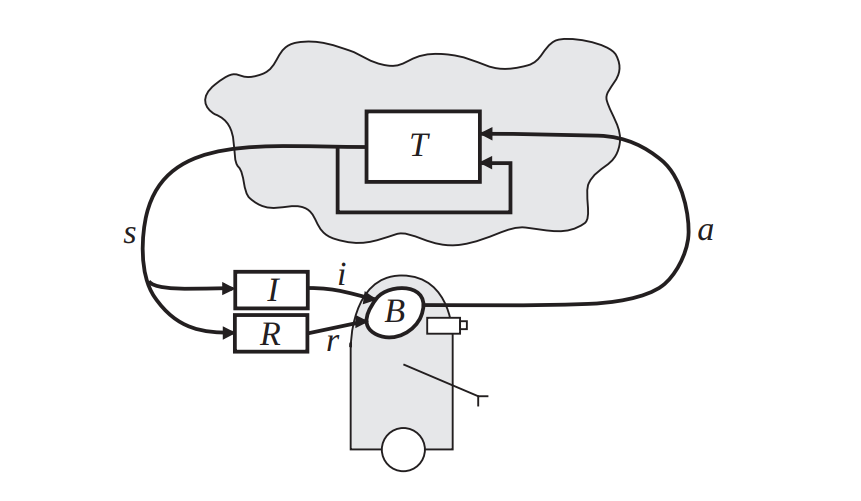
\includegraphics[scale=0.5]{graphics/chapter-2/chap2-rl-overview.png}
    \caption{Tổng quan về học tăng cường}
    \label{fig:chap2-rl-overview}
\end{figure}


Ở một khía cạnh khác, chúng ta có một kỹ thuật khác gọi là học không giám sát. Học không giám sát không có bất kỳ nhãn nào được gán cho dữ liệu, mục tiêu là tìm hiểu một số cấu trúc ẩn của tập dữ liệu hiện có, điển hình là bài toán phân cụm dữ liệu. Học không giám sát khác với học có giám sát ở chỗ đầu ra đúng tương ứng cho mỗi đầu vào là không biết trước. Chúng ta sẽ xem các đối tượng đầu vào như một tập các biến ngẫu nhiên, sau đó tìm cách xây dựng một mô hình mật độ kết hợp cho tập dữ liệu đó. Một phương pháp học tập không giám sát khác đang ngày càng trở nên phổ biến là mạng sinh đối kháng (GANs).

\begin{figure}
    \centering
    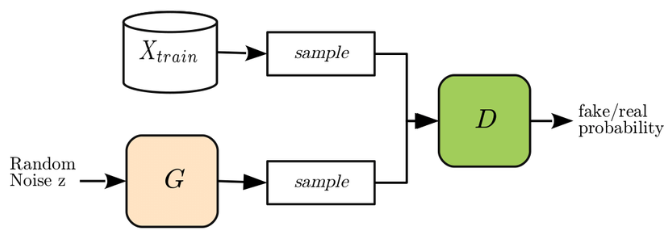
\includegraphics[scale=0.6]{graphics/chapter-2/chap2-gan-overview.png}
    \caption{Tổng quan về học không giám sát sử dụng mạng sinh đối kháng}
    \label{fig:chap2-gan-overview}
\end{figure}


Học tăng cường được nghiên cứu trong đề tài là một phương pháp ở giữa học giám sát và học không giám sát. Nó sử dụng nhiều phương pháp học giám sát đã được thiết kế tốt như mạng nơ-ron sâu dể biểu diễn dữ liệu hoặc làm nền tảng trước khi học tăng cường. Nó có thể tận dụng kinh nghiệm thực tế từ các mô hình đã được huấn luyện bằng học giám sát để quét và tấn công sau đó \cite{liu2020deep}.

% \begin{figure}[!h]
%     \centering
%     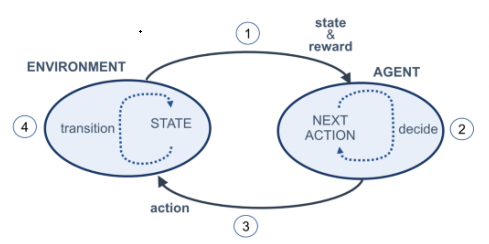
\includegraphics[width=0.9\textwidth]{graphics/chapter-2/chap2-RL_overview.PNG}
%     \caption{Tổng quan về học tăng cường.} 
%     \label{fig:chap2-RL_overview}
% \end{figure}

\subsection{Các thành phần chính}
Mọi lĩnh vực khoa học và kỹ thuật đều có những giả định và hạn chế riêng. Chúng tôi không muốn nói việc học có giám sát là tốt hay không tốt, tuy nhiên có những vấn đề mà học giám sát không thể giải quyết hiệu quả, thay vào đó là học tăng cường. 

Trong học tăng cường, không có các cặp dữ liệu đầu vào và đầu ra đúng, các hành động tối ưu cũng không được đánh giá đúng sai một cách tường mình, thay vào đó là hệ thống phần thưởng nhất định. Hoạt động trực tiếp của tác nhân là thứ được quan tâm. Các vấn đề của học tăng cường liên quan đến việc học những gì cần làm thông qua việc ánh xạ tình huống thành hành động để tối đa hóa phần thưởng bằng số, trong đó có việc tìm kiếm sự cân bằng giữa khám phá (những kiến thức mới chưa được học) và khai thác (những kiến thức đã được học). Nhìn chung, học tăng cường bao gồm 2 thực thể chính là Tác nhân và Môi trường, tương tác với nhau thông qua các kênh giao tiếp của chúng là Hành động, Phần thưởng và Quan sát.


\section{Các nghiên cứu liên quan}

RL không phải là một lĩnh vực mới xuất hiện gần đây, nó đã được nghiên cứu nhiều năm. Các giải pháp có triển vọng trong RL . Ví dụ, RL có thể được sử dụng để tạo ra các phần mềm độc hại mới có khả năng làm sai lệch các đánh giá của các công cụ kiểm như như nghiên cứu của nhóm tác giả Daniel Gibert \cite{gibert2022enhancing} hoặc nhóm tác giả Fang \cite{fang2019evading}. Từ đó cho thấy, các hệ thống thông minh dựa trên RL có tính kinh tế, mạnh mẽ, phổ biến và năng động, đặc biệt là về an ninh mạng do sự thay đổi liên tục của các vec-tơ tấn công và payload của chúng \cite{adawadkar2022cyber}. 


Cho đến nay, đã có một số nghiên cứu liên quan đến các giải pháp tự động hóa kiểm thử thâm nhập bằng cách sử dụng học tăng cường. Trong nghiên cứu của Zhenguo và cộng sự \cite{hu2020automated}, nhóm nghiên cứu đã sử dụng học tăng cường để tìm ra đường tấn công tối ưu nhất cho mô hình mạng thực tế. Các tác giả đã sử dụng công cụ Shodan để thu thập dữ liệu máy chủ thực tế tại các địa điểm công cộng khác nhau để xây dựng các mạng mục tiêu thực tế. Sau đó kết hợp sử dụng MulVAL \cite{yousefi2018reinforcement} và Depth-First Search (DFS) để xây dựng một ma trận tấn công, cuối cùng sử dụng DQN để phân tích ma trận và tìm ra đường tấn công tối ưu nhất cho mô hình mạng. Mặc dù đạt được kết quả tốt theo đánh giá của các tác giả, việc thực hiện vẫn cần rất nhiều sự hỗ trợ từ các framework khác để có thể tự động hóa quá trình thử nghiệm thâm nhập. Trong một nghiên cứu khác, nhóm của Ryusei Maeda \cite{maeda2021automating} cũng đã tập trung vào tấn công tự động với RL sâu, nhưng nghiên cứu này tập trung vào quá trình sau khi bị tấn công. Nghiên cứu này dựa vào một mô-đun agent RL là PowerShell Empire - một mô-đun đã dừng cập nhật - nên nó không thể tiếp tục nghiên cứu và cập nhật sau này.

Ngoài ra, tại hội nghị Arsenal 2018 Black Hat USA, Isao Takaesu đã giới thiệu DeepExploit \cite{takaesudeepexploit}, một công cụ tấn công tự động sử dụng RL để khai thác các lỗ hổng trên máy chủ. Hiện nay, các thành phần của DeepExploit yêu cầu sửa đổi thêm để hoạt động. Không có thông báo về hiệu suất thực tế của nó đối với các lỗ hổng trong thế giới thực.

Lấy cảm hứng từ DeepExploit, trong nghiên cứu này, chúng tôi sử dụng thuật toán A3C \cite{mnih2016asynchronous} để huấn luyện agent RL. Nghiên cứu được phát triển nhằm mục đích tích lũy kinh nghiệm trong việc chọn payload chính xác, để khai thác các lỗ hổng có sẵn trong môi trường tiếp theo. Nghiên cứu tập trung vào quá trình do thám và  tấn công trên máy chủ mục tiêu thông qua Metasploit Framework, là hai giai đoạn đầu tiên của quá trình thử nghiệm thâm nhập \cite{engebretson2013basics}. Ngoài ra, sau quá trình thử nghiệm, công cụ sẽ hỗ trợ xuất các báo cáo về các lỗ hổng bị khai thác một cách trực quan, cho phép người dùng dễ dàng quan sát và đánh giá. Cuối cùng, để đánh giá hiệu suất của mô hình, công cụ kiểm tra thâm nhập tự động được áp dụng cho các kiến trúc mạng nơ-ron khác nhau trong các tình huống kế tiếp. 
